% \section{Results}

\noindent
\subsection{RQ1: Performance of supervised fine-tuning for refactoring}

The research question aims to evaluate the performance of the fine-tuned models
for the refactored code generation.
The first part of Table~\ref{tab:all_metrics}
(\ie{} \textsc{pt + sft} column)
presents the results obtained by the considered models for the refactored code generation task. 
The results presented in the table demonstrate that the \plbart{} model outperforms other models metrics and code-specific evaluation measures. Specifically, \plbart{} achieves the highest scores on the \bleu{} and \rouge{} metrics, which assess the lexical and semantic similarity of the generated text to the ground truth. Crucially, \plbart{} also exhibits superior performance on the \codebleu{} metric, which captures the syntactic and structural fidelity of the generated code snippets.

\begin{table}[ht!]
    \centering
    \caption{Experimental results for different learning objectives. Here, PT, SFT, and RL refer to pre-trained, supervised fine-tuned, and reinforcement learning-based models}
    \resizebox{\columnwidth}{!}{
        \begin{tabular}{cccc|ccc|ccc}
        \toprule
        \multirow{2}{*}{Models} & \multicolumn{3}{c}{PT + SFT (RQ1)} & \multicolumn{3}{c}{PT + RL (RQ2)} & \multicolumn{3}{c}{PT + SFT + RL (RQ3)} \\
        \cmidrule(lr){2-4}
        \cmidrule(lr){5-7}
        \cmidrule(lr){8-10}
        & \makecell[c]{BLEU} & \makecell[c]{ROUGE} &\makecell[c]{CodeBLEU} & \makecell[c]{BLEU} & \makecell[c]{ROUGE} &\makecell[c]{CodeBLEU} & \makecell[c]{BLEU} & \makecell[c]{ROUGE} &\makecell[c]{CodeBLEU} \\
        \midrule
        \makecell[l]{Code-T5} & \makecell[c]{$67.80$} & \makecell[c]{$77.49$} &\makecell[c]{$53.13$} & \makecell[c]{$38.80$} & \makecell[c]{$37.62$} & \makecell[c]{$31.99$} & \makecell[c]{$\textbf{$75.91$\textsuperscript{$\bigstar$}}$} & \makecell[c]{$\textbf{$79.92$\textsuperscript{$\bigstar$}}$} & \makecell[c]{$\textbf{$61.87$\textsuperscript{$\bigstar$}}$} \\ \addlinespace
        \makecell[l]{PLBART} & \makecell[c]{$\textbf{68.28}$} & \makecell[c]{$\textbf{80.62}$} &\makecell[c]{$\textbf{55.66}$} & \makecell[c]{$30.21$} & \makecell[c]{$29.56$} & \makecell[c]{$22.48$} & \makecell[c]{$71.20$} & \makecell[c]{$69.68$} & \makecell[c]{$58.17$} \\ \addlinespace
        \makecell[l]{CodeGPT-adapt} & \makecell[c]{$62.68$} & \makecell[c]{$65.76$} &\makecell[c]{$49.29$} & \makecell[c]{$27.68$} & \makecell[c]{$30.76$} & \makecell[c]{$20.29$} & \makecell[c]{${64.96}$} & \makecell[c]{${67.82}$} & \makecell[c]{${47.99}$} \\ \addlinespace        
        \makecell[l]{CodeGen} & \makecell[c]{$59.32$} & \makecell[c]{$63.74$} &\makecell[c]{$42.11$} & \makecell[c]{$34.32$} & \makecell[c]{$33.74$} & \makecell[c]{$27.11$} & \makecell[c]{${61.59}$} & \makecell[c]{${60.52}$} & \makecell[c]{${46.67}$} \\
        \bottomrule
        
        \end{tabular}
    }
    
    \label{tab:all_metrics}
\end{table}

Furthermore, a comparative analysis reveals that \plbart{} substantially outperforms the \codetf{} model, achieving a $4.54\%$ higher \codebleu{} score. The performance gap is even more pronounced when contrasted with the \codegpt{} model, for which \plbart{} demonstrates an $12.98\%$ improvement on the \codebleu{} metric. These findings suggest that the \plbart{} model was successful in generating extract method refactored outputs that closely resemble the ground truth in terms of syntactic correctness.


To gain a more thorough understanding of the validity and robustness of the generated refactored outputs, additional validation checks and analyses are necessary. As detailed in Section~\ref{subsubsection:qualitative}, we
create a manually validated dataset for qualitative evaluation.
The dataset contains $122$ samples with before and after refactored code and corresponding test cases.
We use this qualitative dataset to check whether the trained model generates code without any syntactic and compilation errors, whether the generated code has extract method refactoring, and to what extent the generated code is passing the test cases.
Table~\ref{tab:exresults} presents the obtained results. 
For RQ1, notably, fine-tuned \codetf{} achieved the highest performance in qualitative evaluation. This supports our assertion that relying solely on quantitative metrics may yield misleading results and potentially produce low-quality refactored code.


\begin{boxH}
\textbf{RQ1 Summary:}
Fine tuning code \llm{}s show  an effective way to teach language models to generate refactored code automatically. Specifically, \plbart{} outperform other models in all the considered metrics. It show significant improvements over \codetf{} and \codegpt{}, particularly in \codebleu{} scores. 
% 74\% of \plbart{}'s outputs in the validation dataset exhibited desirable syntactic properties.
However, qualitative evaluation reveals that \codetf{} performs best in generating syntactically correct and functionally valid refactored code. 
% \todo{add qualitative results summary-DONE}
\end{boxH}


% \vspace{3mm}
\subsection{RQ2: Effectiveness of reinforcement learning for automated refactoring}

This research question aims to evaluate the application of \rl{} on the refactoring task when applied on pre-trained \llmsc{}.
The second part of the Table~\ref{tab:all_metrics} (\ie{} PT + RL column) shows
the obtained results.
Our results show that \codetf{} model demonstrates superior performance across all evaluation metrics compared to other language models when trained using \rl{}.

Interestingly, unlike the results observed in RQ1 with traditional fine-tuning, direct fine-tuning using \rl{} with Proximal Policy Optimization (\ppo{}) does not perform well.
% across all models. \todo{how did we know this? We dont have the results from the baseline (pure pre-trained models)
% But this is in comparison to the direct fine tuned models for which results are there in Table 2}
This outcome may be attributed to the complexity of the \exm{} refactoring task and the potential mismatch between the \rl{} objective and the nuanced requirements of code refactoring. Fine-tuning language models that have been pre-trained on tasks other than code refactoring directly using non-differentiable rewards poses challenges. The disparity between the pre-training task and the target task of code refactoring makes it difficult to effectively train the models using \rl{} techniques. 

\begin{table}[ht!]
\centering
\caption{Qualitative evaluation of fine tuned models}
\label{tab:exresults}
\rowcolors{2}{gray!25}{white}
\begin{tabular}{p{1cm}p{4cm}|%.5
>{\raggedleft\arraybackslash}p{2.5cm}%
>{\raggedleft\arraybackslash}p{2cm}%
>{\raggedleft\arraybackslash}p{2cm}%
>{\raggedleft\arraybackslash}p{2cm}%
>{\raggedleft\arraybackslash}p{2cm}%
}
&\textbf{Models} & \textbf{Syntactically correct (\%)}  & \textbf{Refactoring detected (\%)} & \textbf{Compile successfully (\%)} & \textbf{\# of unit tests passed (out of $122$)} \\ \midrule
&Code-T5 (FT) & $ \textbf{78.6} $  & $\textbf{66.4}$ & $\textbf{72.1}$ & $\textbf{41}$ \\
&PLBART (FT) & $76.9$ & $63.8$ & $69.5$ & $38$ \\
&CodeGPT-adapt (FT) & ${77.5}$ & ${64.3}$ & ${70.1}$ & $39$ \\
\multirow{-4}{*}{RQ1}&CodeGen (FT) & $78.3$ & ${65.1}$ & $71.2$ & $40$ \\ \midrule
&Code-T5 + RL & {21.4}  & {20.2} & {22.3} & {21} \\
&PLBART + RL & ${21.7}$ & ${18.9}$ & ${21.5}$ & ${16}$ \\
&CodeGPT-adapt + RL& ${19.7}$ & ${14.1}$ & ${20.2}$ & $14$ \\
\multirow{-4}{*}{RQ2}&CodeGen + RL & $23.6$ & ${19.2}$ & $21.1$ & $9$ \\ 
\midrule
&Code-T5 (FT) + RL & $\mathbf{85.7}$  & $\mathbf{74.9}$ & $\mathbf{79.8}$ & $\mathbf{66}$ \\
&PLBART  (FT) + RL & ${82.4}$ & ${71.6}$ & ${76.3}$ & ${58}$ \\
&CodeGPT-adapt  (FT) + RL& ${83.1}$ & ${72.2}$ & ${77.5}$ & $61$ \\
\multirow{-4}{*}{RQ3}&CodeGen  (FT) + RL & $84.3$ & ${73.5}$ & $78.6$ & $63$ \\ \bottomrule

\end{tabular}
\end{table}


Qualitatively also, as shown in \textit{RQ2} of Table~\ref{tab:exresults}, the generated refactorings exhibit poor quality. 

The \rl{} method's poor performance in functional areas highlights a misalignment with the refactored code's true requirements. This suggests that the \rl{} reward signals may insufficiently penalize syntactic and semantic errors, resulting in models 
% that excel in surface-level metrics but fail 
to produce functionally valid code. A potential explanation for this behavior could be that the \rl{}, performed on a generic pretrained language model, may not receive appropriate reward signals from our reward framework or the non-score rewards (KL divergence penalty). This hypothesis can be corroborated by examining Figure~\ref{fig:rl_stats}. Figure~\ref{fig:std_reward} illustrates the persistent high standard deviation of rewards for the \rl{} fine-tuned model throughout increasing training steps. This trend indicates that the reward signals fail to effectively steer the model towards optimal performance. Concurrently, Figure~\ref{fig:kl_penalty} reveals an upward trajectory in the KL-Divergence penalty over time. This escalation suggests a growing divergence between the trained model and the reference model, further supporting our hypothesis that the current reward system may be inadequate for guiding the model towards generating functionally sound code refactorings. 


\begin{boxH}
\textbf{RQ2 Summary:} Generating refactored code from a pre-trained model directly aligned with \rl{} does not produce comparable results to the corresponding fine-tuned models as shown in RQ1 quantitatively or qualitatively.

\end{boxH}





\subsection{RQ3: Evaluating the performance of reinforcement learning and fine-tuned LLMs for refactoring} 

In this research question, we aim to evaluate the efficacy of applying \rl{} to generate refactored code, focusing on model performance when fine-tuned using a combination of supervised fine-tuning (\textsc{sft}) and \rl{} objectives.
Specifically, we start with the trained fine-tuned models from RQ1, and train them with \ppo{} and reward from a feedback system to observe any improvements in the models compared to their fine-tuned counterparts.
% Our study investigated the efficacy of applying \rl{} to generate refactored code, focusing on model performance when fine-tuned using a combination of supervised fine-tuning (\textsc{SFT}) and \textsc{DRL} objectives. In RQ1, we examined the impact of maximizing the log-likelihood of the next correct code through \textsc{SFT}. RQ2 explored the effects of \textsc{DRL}, which aims to maximize the reward signal using a policy-based approach to select the optimal policy.

Table~\ref{tab:all_metrics} presents the results in the column titled PT + SFT + RL
along with results obtained in other settings as discussed in RQ1 and RQ2.
The results demonstrate that \textbf{the most effective outcomes are achieved when models are trained using both SFT and RL objectives.} This combined approach lead to significant improvements across various metrics. Specifically, we observed an approximate 10\% increase in \codebleu{} compared to models trained solely with \textsc{sft}, and an 11\% improvement over those trained exclusively with \rl{}. Similar performance gains were noted in other metrics, including \bleu{} and \rouge{}.
The superiority of the combined approach can be attributed to the complementary nature of \textsc{sft} and \textsc{rl}. \textsc{sft} excels at identifying inherent patterns and structures within data, primarily utilizing large labeled datasets. In contrast, \textsc{rl} adapts through environmental interactions, optimizing predefined reward metrics. By integrating these methodologies, our model can effectively navigate dynamic contexts while capturing underlying data patterns.

Our combined approach demonstrated a significant improvement in the evaluated quality metrics. The number of successfully passing test cases increased substantially, rising from $41$ in the best-performing model, \codetf{}, to $66$---a significant improvement of approximately $61\%$. Additionally, RefactoringMiner identified an increased number of cases, from $87$ to $98$. These results highlight the efficacy of \rl{} in producing accurate extract method refactored code.

Figure~\ref{fig:rl_stats} illustrates the trends in the standard deviation of rewards and the KL-Divergence penalty across training steps. The initial decline in standard deviation, followed by stabilization, coupled with consistent KL-divergence penalties, suggests that our reward modeling strategy effectively aligns a fine-tuned language model for the extract method refactoring task. These results collectively highlight the efficacy of \rl{} in producing accurate extract method refactored code.

\begin{figure*}[ht!]
    \centering
    \begin{subfigure}[t]{0.45\textwidth}
        \centering
        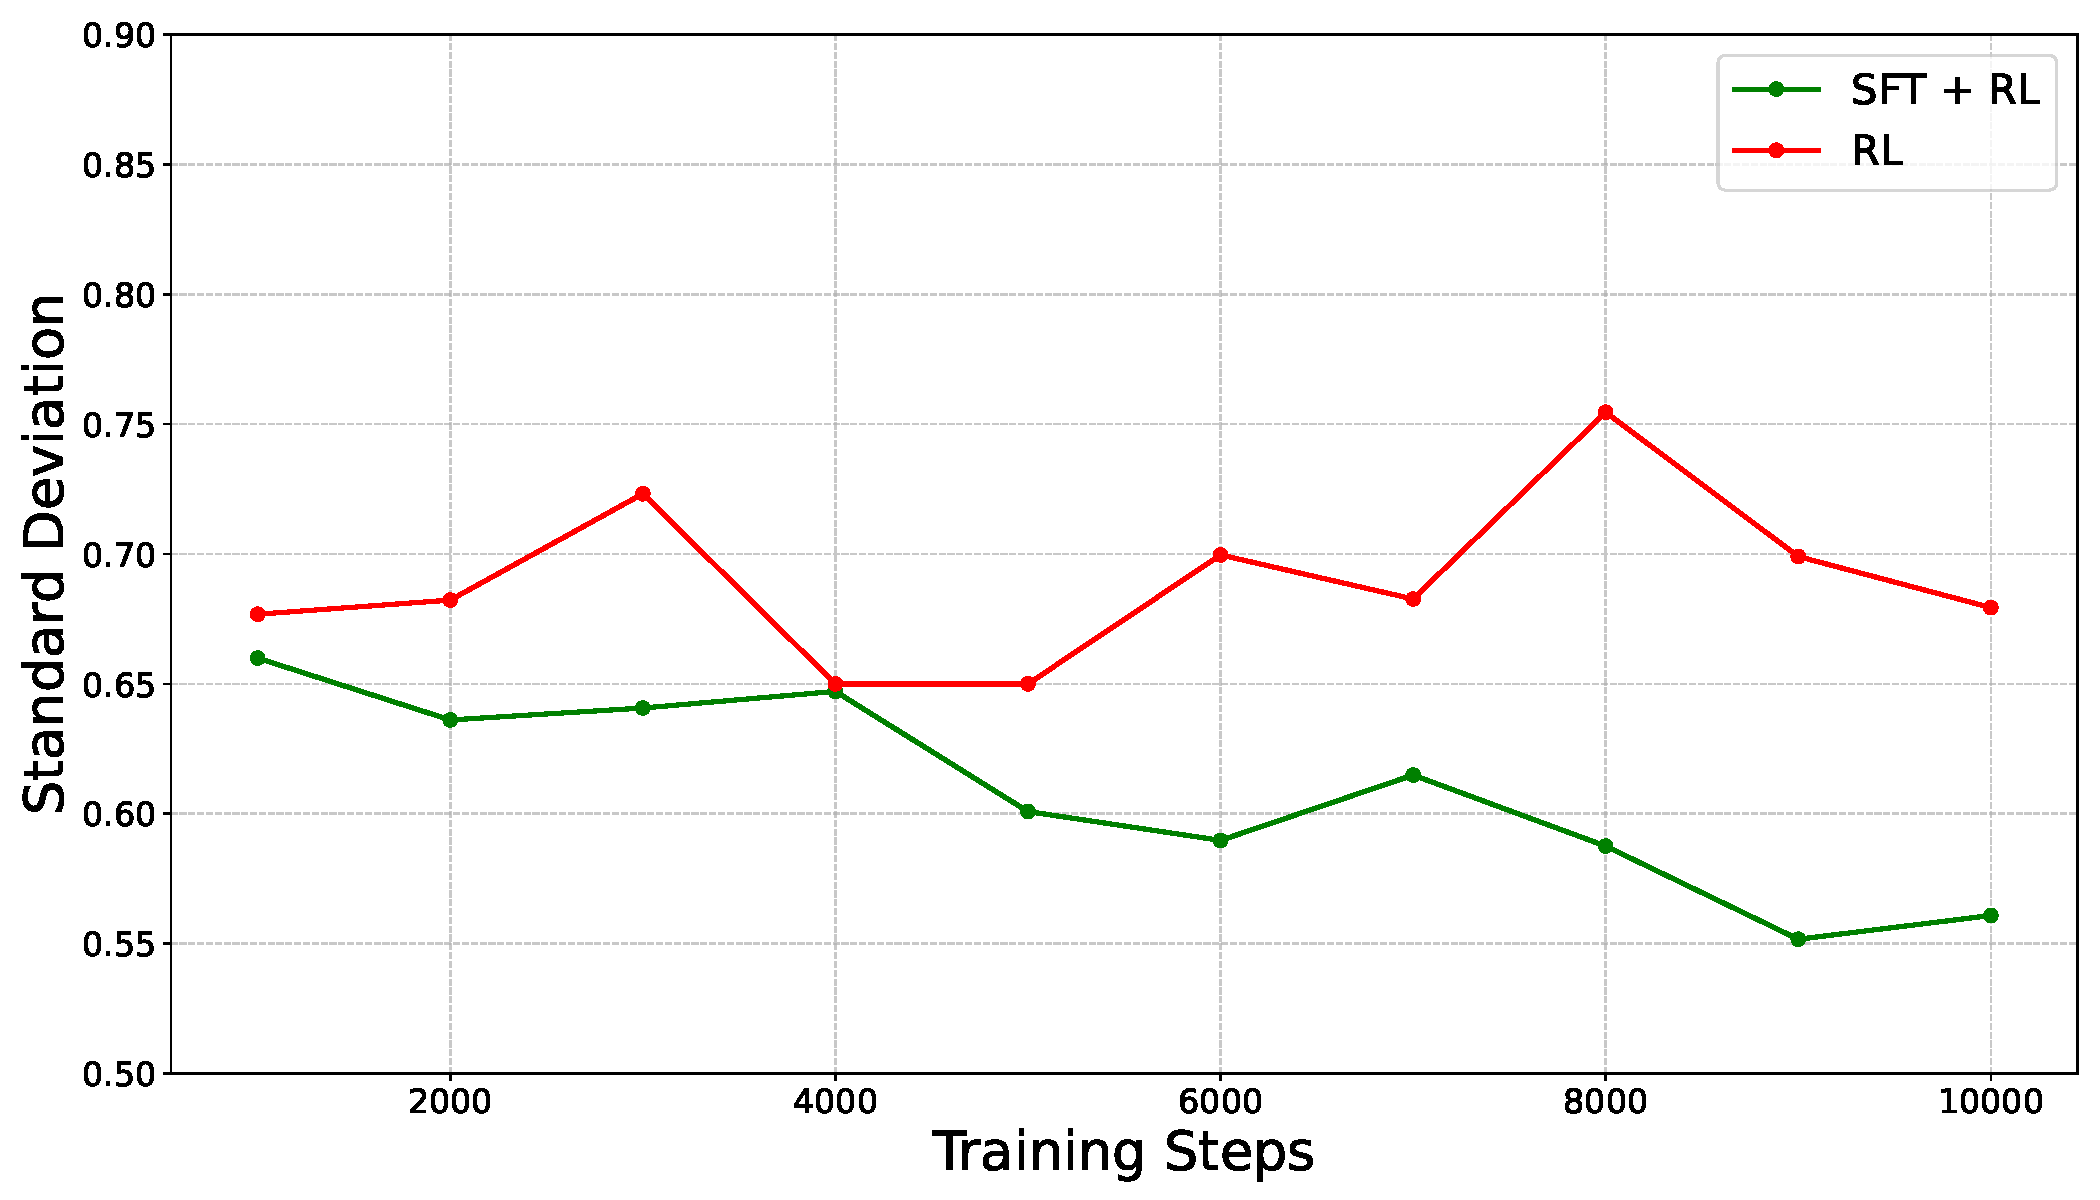
\includegraphics[height=1.5in]{chapters/generation/images/std_reward.pdf}
       \caption{Standard Deviation of Rewards}
        \label{fig:std_reward}
    \end{subfigure}
 ~
    \begin{subfigure}[t]{0.45\textwidth}
        \centering
        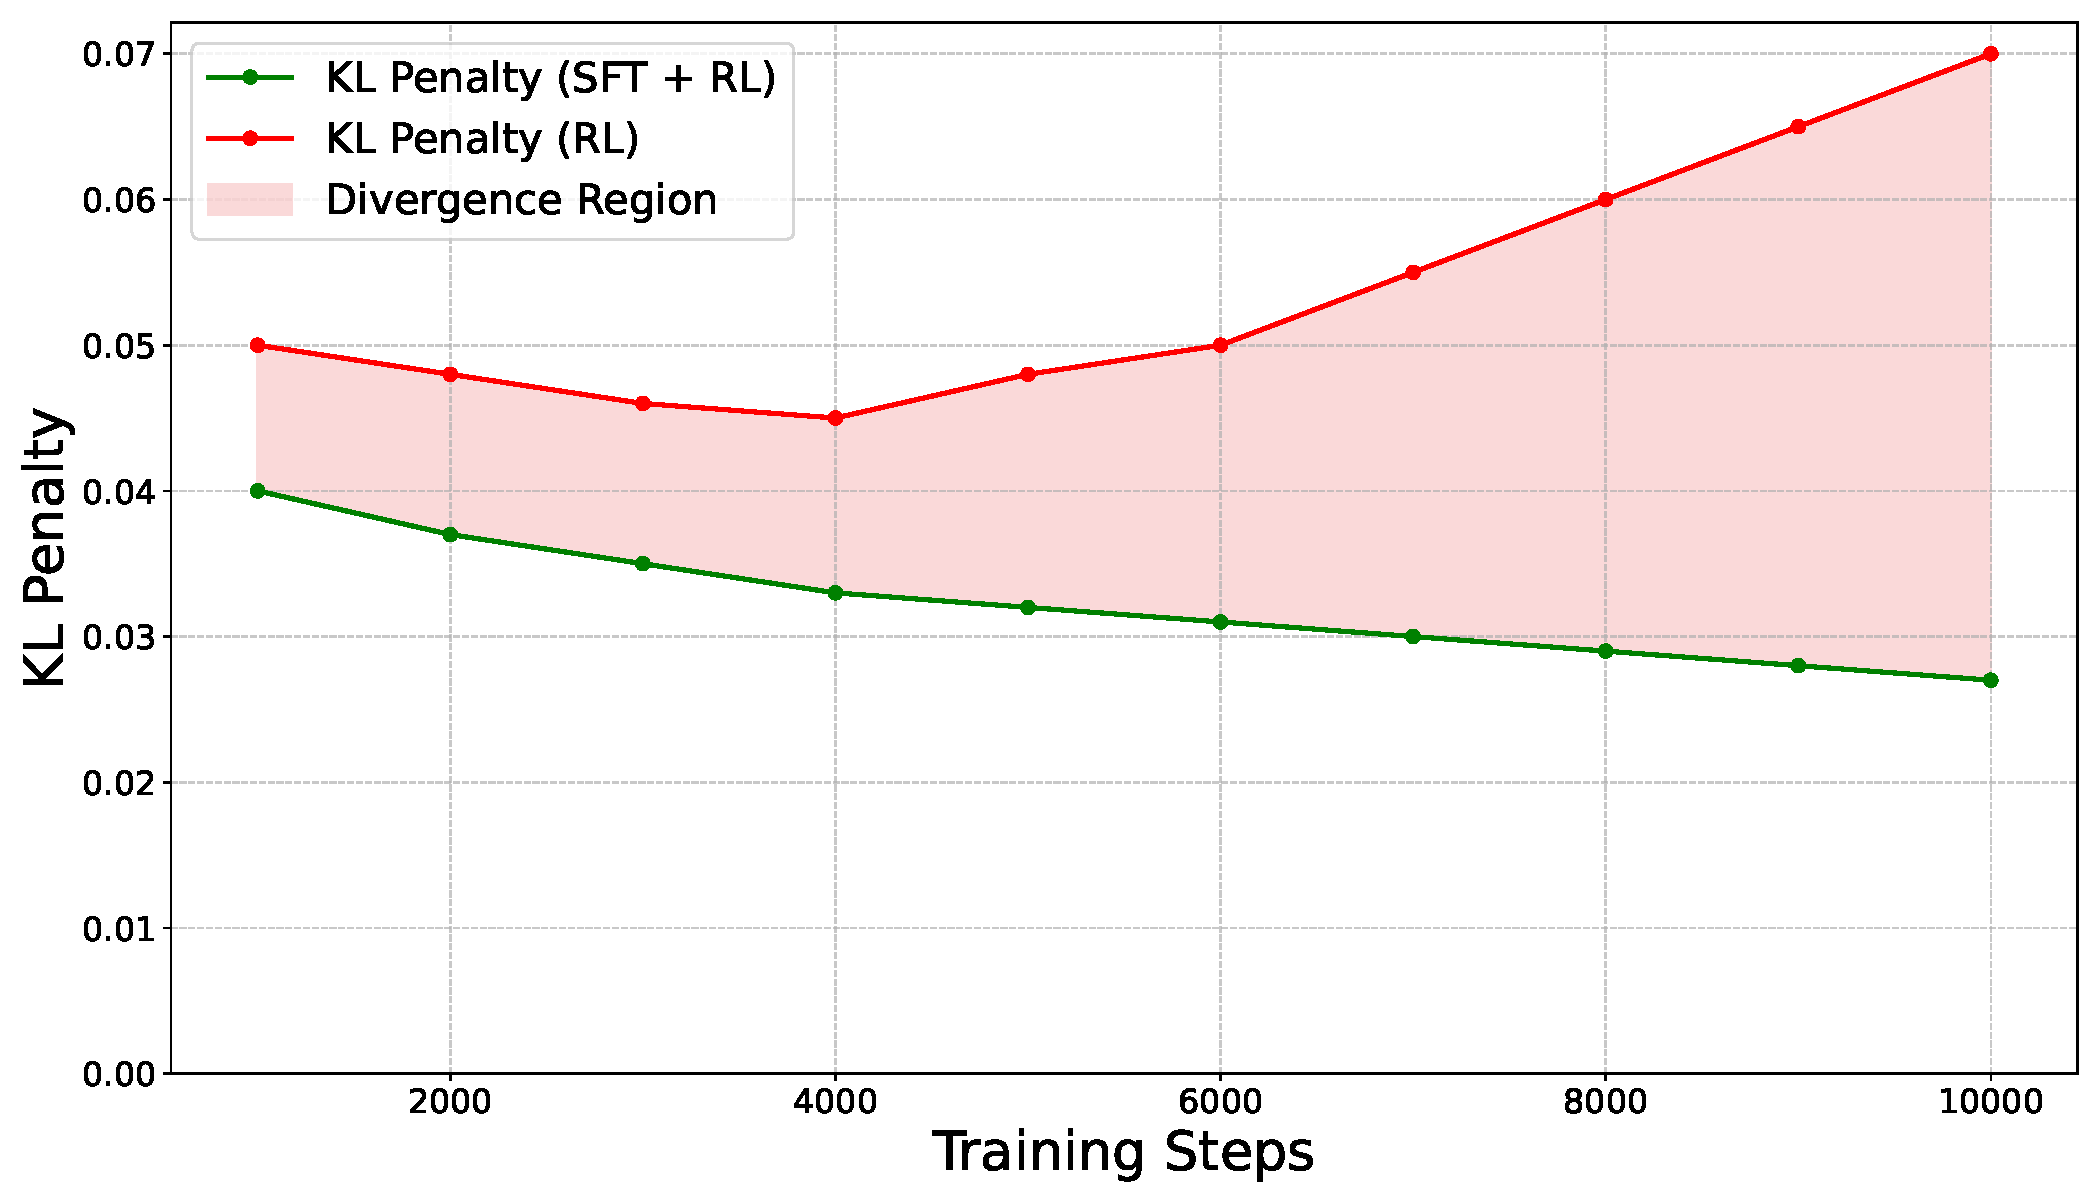
\includegraphics[height=1.5in]{chapters/generation/images/kl_penalty.pdf}
        \caption{Negated KL Divergence Penalty}
        \label{fig:kl_penalty}
    \end{subfigure}
    \caption{RL training observations}
    \label{fig:rl_stats}
\end{figure*}


While \textsc{sft} typically learns based on loss derived from labeled data, the integration with \textsc{rl} allows the model to benefit from a more comprehensive feedback system, including reward signals. This holistic approach contributes to the observed performance enhancements.

We present an illustrative example of a \exm{} refactoring in Figure~\ref{fig:example}, highlighting the differences of \sft{} and \rl{} techniques.
The original method belongs to \texttt{aws/aws-dynamodb-encryption\-java} repository as present in commit \texttt{ea43801}. 
Snippets \texttt{B} and \texttt{C} are generated by \sft{} model and combined \sft{} with \rl{} aligned models respectively. As we can see from the generated example, there are few syntactic errors (highlighted by red background color) present in the output generated by the fine-tuned only model. The combined \rl{} model seems to be more aligned to the ground truth. However, the generated code is not absolutely accurate because at line $10$ it throws an \texttt{IllegalArgumentException} instead of \texttt{IndexOutOfBoundException}. But this example strengthens our claims that the combined \sft{} model with \rl{} alignment enhances language model performance to generate more accurate extract method refactored code.

\begin{figure*}[ht!]
    \centering
    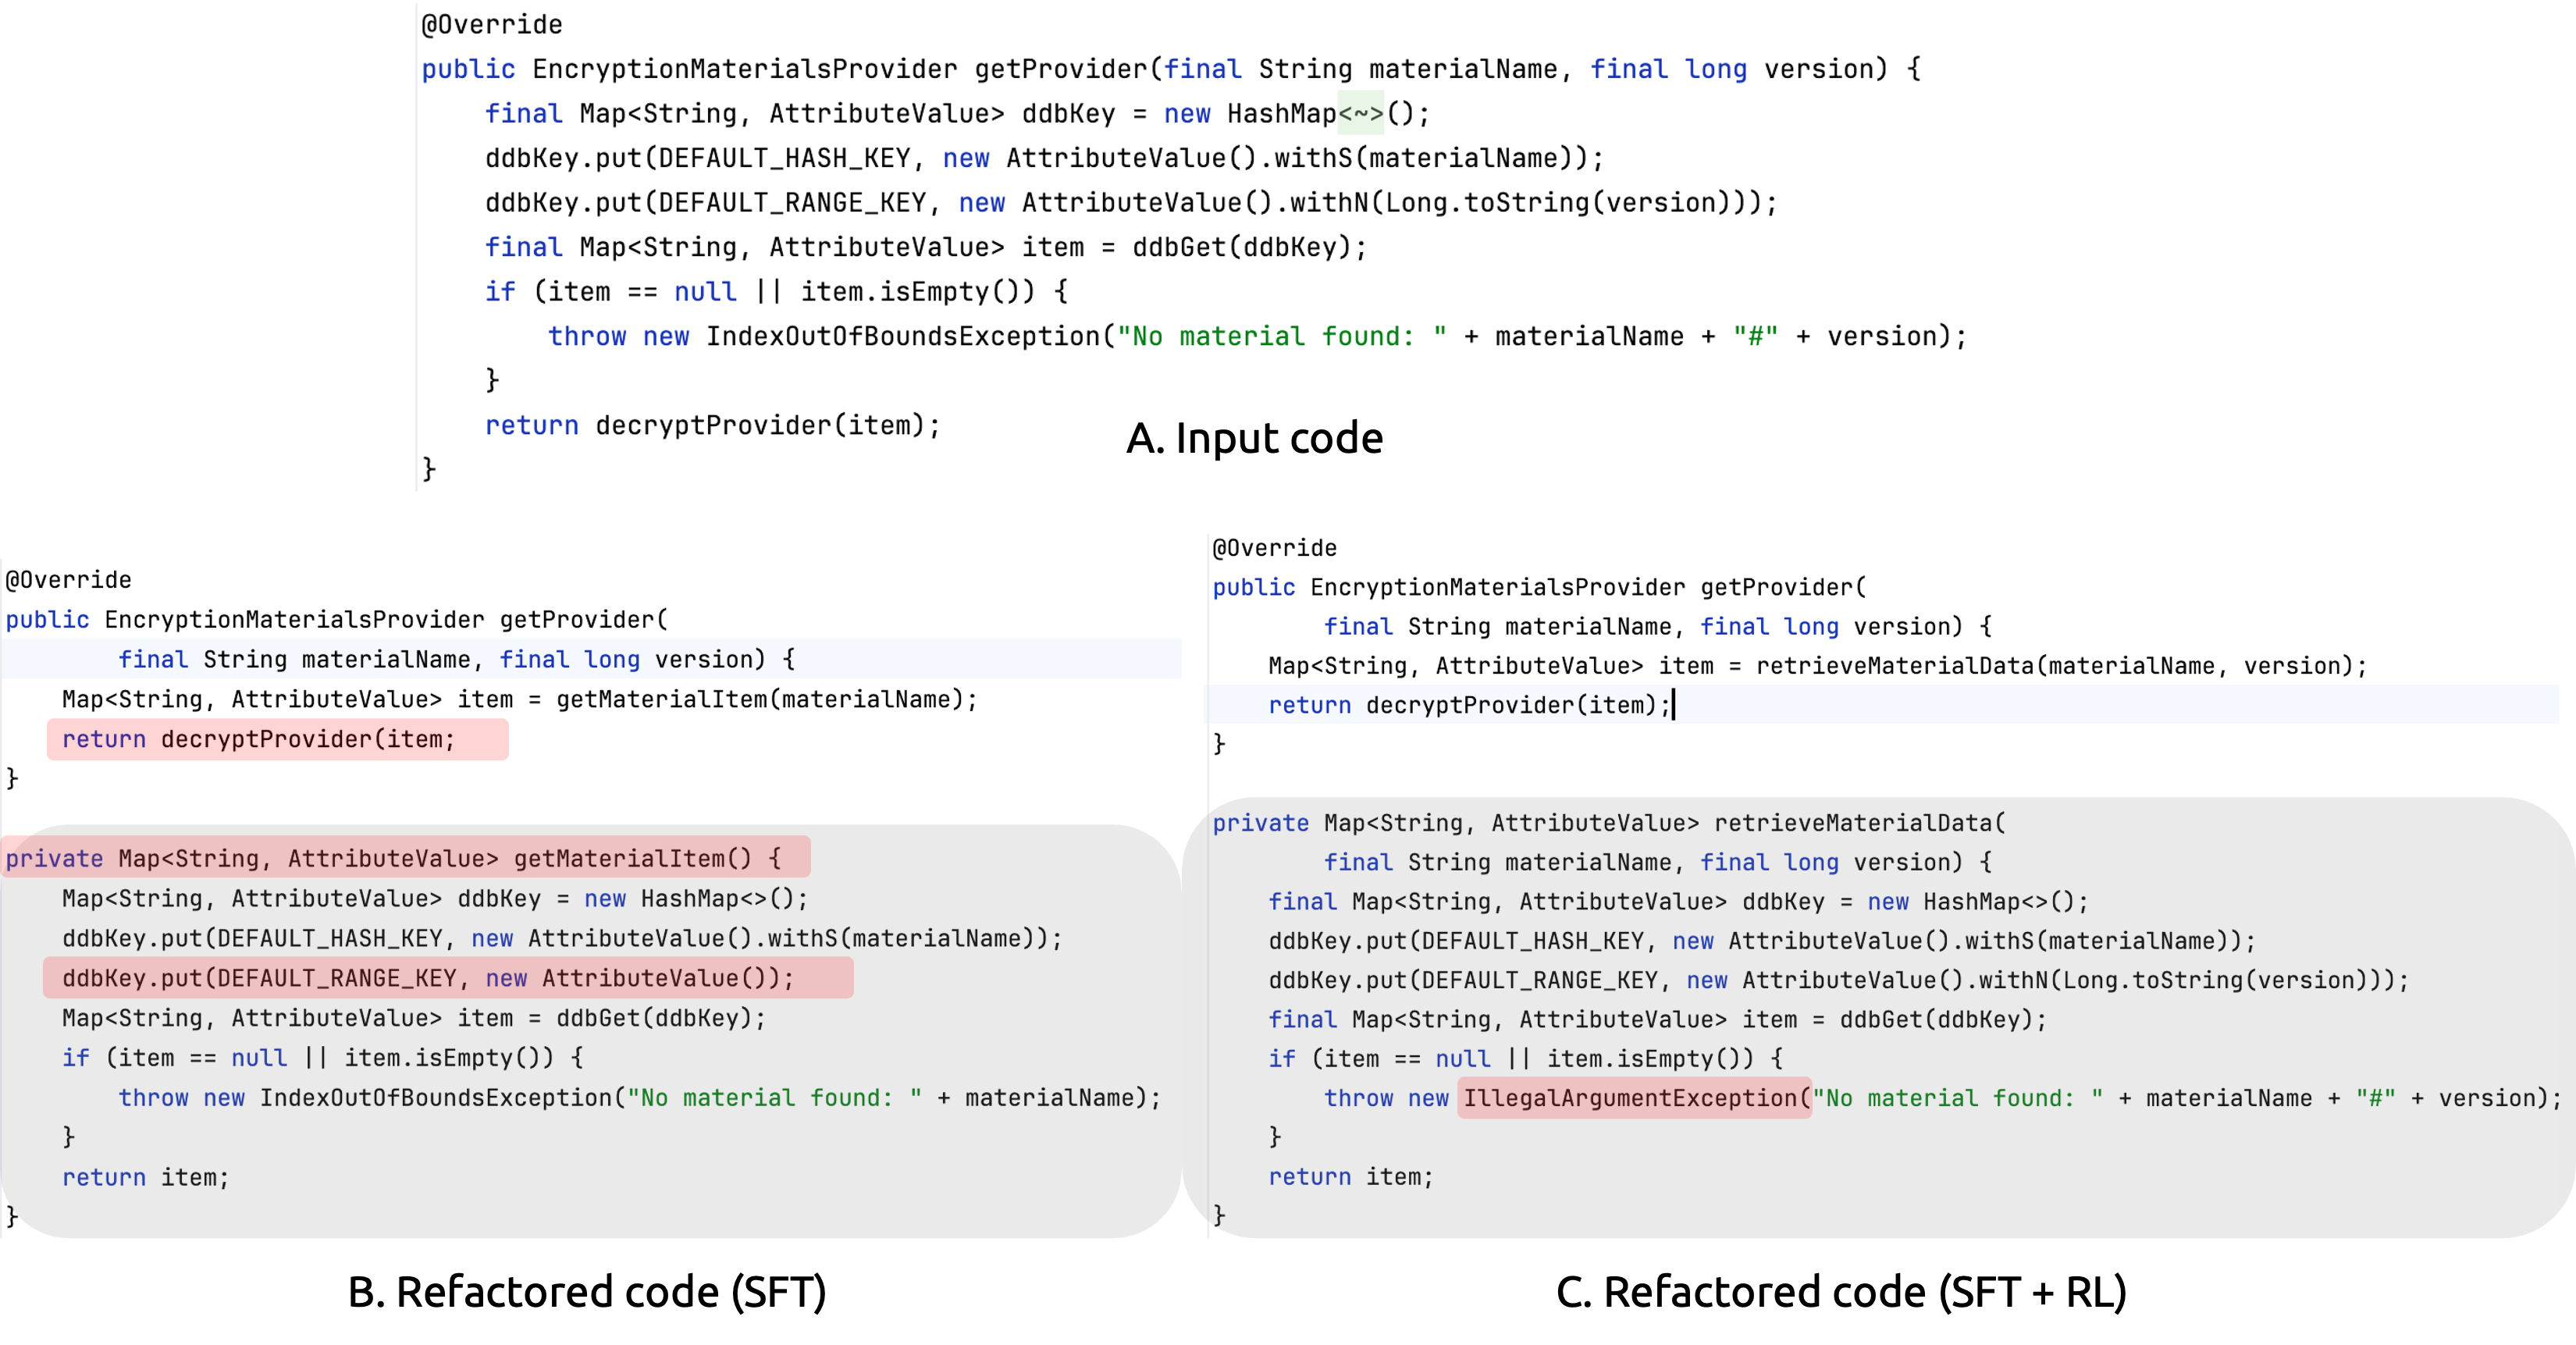
\includegraphics[width=\textwidth]{chapters/generation/images/example.png}
    \caption{Extract method refactoring example generated using Supervised Fine-Tuning (SFT) and the combination of SFT and Reinforcement Learning (RL) techniques}
    \label{fig:example}
\end{figure*}

\begin{boxH}
    \textbf{RQ3 Summary:} Our results demonstrates that combining supervised fine-tuning and \rl{} objectives yields superior results in generating refactored code. This integrated approach outperforms individual methods, showing significant improvements in \codebleu{}, \bleu{}, and \rouge{} metrics, while mitigating common limitations associated with single-objective training.
\end{boxH}
